\documentclass[tikz,border=6pt]{standalone}
% Shared publication style for the standalone paper figures.
% All colours are from the colour-blind-safe Okabe--Ito palette.
\usepackage{amsmath,amssymb,bm}
\usepackage{pgfplots}
\usepackage{pgfplotstable}
\usetikzlibrary{arrows.meta,calc,fit,positioning,backgrounds}
\usepgfplotslibrary{groupplots,fillbetween}
\pgfplotsset{compat=1.18}

\definecolor{oiBlue}{HTML}{0072B2}
\definecolor{oiSky}{HTML}{56B4E9}
\definecolor{oiGreen}{HTML}{009E73}
\definecolor{oiOrange}{HTML}{E69F00}
\definecolor{oiVermillion}{HTML}{D55E00}
\definecolor{oiPurple}{HTML}{CC79A7}
\definecolor{ink}{HTML}{20252B}
\definecolor{midgray}{HTML}{6B7280}
\definecolor{lightgray}{HTML}{D7DCE2}
\definecolor{panelgray}{HTML}{F4F6F8}

\pgfplotsset{
  paper axis/.style={
    axis line style={draw=ink,line width=0.45pt},
    tick style={draw=ink,line width=0.4pt},
    tick label style={font=\scriptsize,text=ink},
    label style={font=\small,text=ink},
    title style={font=\small\bfseries,text=ink,yshift=1pt},
    legend style={
      font=\scriptsize,
      draw=none,
      fill=none,
      cells={anchor=west},
      /tikz/every even column/.append style={column sep=4pt}
    },
    grid style={draw=lightgray,line width=0.35pt},
    major grid style={draw=lightgray,line width=0.35pt},
    every axis plot/.append style={line width=1.05pt},
    clip marker paths=true,
    scale only axis
  },
  paper mark/.style={mark size=2.0pt,line width=0.9pt},
}

\tikzset{
  every node/.style={text=ink},
  flow arrow/.style={-{Stealth[length=2.2mm,width=1.5mm]},line width=0.9pt,draw=ink},
  support arrow/.style={-{Stealth[length=2mm,width=1.4mm]},line width=0.8pt,draw=midgray},
  theorem box/.style={
    rounded corners=2pt,
    draw=oiBlue,
    fill=oiBlue!7,
    line width=1.1pt,
    align=center,
    inner sep=5pt
  },
  corollary box/.style={
    rounded corners=2pt,
    draw=oiGreen!85!black,
    fill=oiGreen!6,
    line width=0.8pt,
    align=center,
    inner sep=4pt
  },
  support box/.style={
    rounded corners=2pt,
    draw=midgray,
    fill=panelgray,
    line width=0.7pt,
    align=center,
    inner sep=4pt
  },
  source box/.style={
    rounded corners=2pt,
    draw=oiOrange!90!black,
    fill=oiOrange!8,
    line width=0.8pt,
    align=center,
    inner sep=4pt
  },
  arrow label/.style={font=\scriptsize,fill=white,inner sep=1.2pt,text=midgray},
  panel label/.style={font=\small\bfseries,anchor=north west,text=ink},
}


\begin{document}
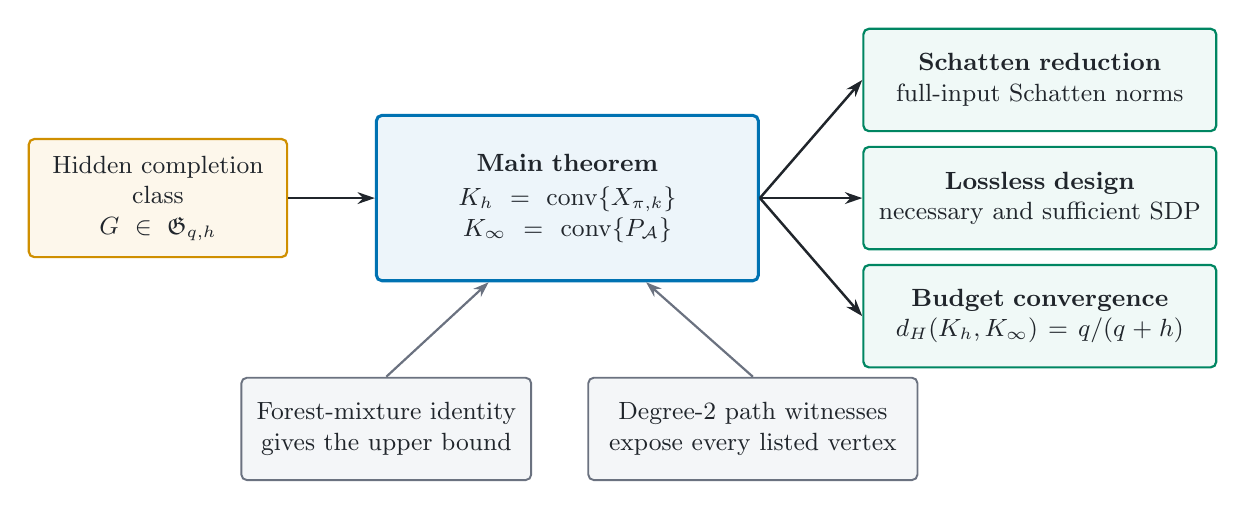
\begin{tikzpicture}[font=\small,node distance=7mm and 11mm]
  \node[source box,text width=30mm,minimum height=15mm] (completion) {
    Hidden completion\\class\\
    $G\in\mathfrak G_{q,h}$
  };

  \node[theorem box,right=11mm of completion,text width=45mm,minimum height=21mm] (main) {
    \textbf{Main theorem}\\[1.5pt]
    $K_h=\operatorname{conv}\{X_{\pi,k}\}$\\
    $K_\infty=\operatorname{conv}\{P_{\mathcal A}\}$
  };

  \node[corollary box,right=13mm of main,yshift=15mm,
        text width=42mm,minimum height=13mm] (schatten) {
    \textbf{Schatten reduction}\\
    full-input Schatten norms
  };
  \node[corollary box,right=13mm of main,
        text width=42mm,minimum height=13mm] (sdp) {
    \textbf{Lossless design}\\
    necessary and sufficient SDP
  };
  \node[corollary box,right=13mm of main,yshift=-15mm,
        text width=42mm,minimum height=13mm] (rate) {
    \textbf{Budget convergence}\\
    $d_H(K_h,K_\infty)=q/(q+h)$
  };

  \node[support box,below=12mm of main,xshift=-23mm,
        text width=34mm,minimum height=13mm] (forest) {
    Forest-mixture identity\\
    gives the upper bound
  };
  \node[support box,right=7mm of forest,
        text width=39mm,minimum height=13mm] (paths) {
    Degree-2 path witnesses\\
    expose every listed vertex
  };

  \draw[flow arrow] (completion.east) -- (main.west);
  \draw[flow arrow] (main.east) -- (schatten.west);
  \draw[flow arrow] (main.east) -- (sdp.west);
  \draw[flow arrow] (main.east) -- (rate.west);
  \draw[support arrow] (forest.north) -- ([xshift=-10mm]main.south);
  \draw[support arrow] (paths.north) -- ([xshift=10mm]main.south);

\end{tikzpicture}
\end{document}
